\documentclass[11pt,a4j]{jsarticle}

\usepackage{float,array,booktabs,here}
\usepackage{amsmath}
\usepackage[dvipdfmx]{graphicx}
\usepackage[top=20truemm,bottom=25truemm,left=20truemm,right=20truemm]{geometry}
\usepackage{url}
\usepackage{listings}

\lstset{language=POV,frame=single, stepnumber=1,numbersep=2pt,tabsize=2,%
basicstyle=\verysmall\ttfamily, stringstyle=\small\texttt, commentstyle=\slshape, captionpos=b,%
columns=[l]{fullflexible}}

\makeatletter
\newcommand{\figcaption}[1]{\def\@captype{figure}\caption{#1}}
\newcommand{\tblcaption}[1]{\def\@captype{table}\caption{#1}}
\makeatother

\newcommand{\Maru}[1]{\ooalign{
\ifnum#1<10 \hfil\resizebox{.9\width}{.85\height}{#1}\hfil
\else
\hfil\resizebox{.6\width}{.8\height}{#1}\hfil
\fi
\crcr
\raise.1ex\hbox{$\bigcirc$}}}

%\usepackage[tableposition=top]{caption}



\begin{document}

 % \title{コンピュータグラフィックス}
% \author{hogehoge}
% \date{2015年5月9日}
 % \maketitle


\section{目的}
POV-Rayを使用し物体や視点及び光源などをスクリプトで記述しモデリングを行い、
レイトレーシング法において必要な要素と考え方を理解する。
また与えられたテーマに従い、CG作品を制作する。


\section{モデリング}
\label{sec:モデリング}

家電というテーマに対して、私は、現代的なデザインといえるダイソンの扇風機を題材にした。
シンプルさを出すために、周りに環境を用意するのでなく、商品紹介のような、白い世界の中にモデリングした
扇風機を配置した。

\subsection{光源}
光源は4つの光源を配置して、なるべく綺麗に見えるように配置した。


\subsection{送風部}

送風部はCSGを用いて作成した。以下にCSG木を示す。
\vspace{15cm}


\subsection{筒部}

CSG木を用いて作成した。いかにCSG木を示す。
\vspace{15cm}





\section{シーンファイル}
\label{sec:シーンファイル}

以下に、今回作成したモデルのシーンファイルを添付する。

\begin{lstlisting}[basicstyle=\ttfamily\footnotesize, frame=single]
#include "colors.inc"
#include "shapes.inc"
#include "textures.inc"

camera{
  location <15,7,13>
  look_at<0,2.5,0>
  angle 20
}
light_source{<15,1,15> color 1*White}
light_source{<6,20,0> color 2*White}
light_source{<-6,20,0> color 2*White}
light_source{<0,3.5,0> color 0.3*White}
light_source { <15, 7, 15>
	color White
	spotlight
	point_at <-1.5,3.5,0>
	radius 2
	falloff 10
	tightness 20
}
#declare fan =
union{ // fan
	union{
		difference{
			object{
				cylinder{<0,3.5,-0.4>,<0,3.5,0.3>,1.5
			 		pigment{ color Gray05}
				}
			}
     		 	object{
				cylinder{<0,3.5,-1>,<0,3.5,1>,1.49}
		 		pigment{ color Gray05}
			}
    }
		difference{
			object{
				cylinder{<0,3.5,-0.5>,<0,3.5,-0.48>,1.5
			 		pigment{ color Gray05}
				}
			}
     		 	object{
				cylinder{<0,3.5,-1>,<0,3.5,1>,1.35}
		 		pigment{ color Gray05}
			}
  	}
		difference{
			object{
				cylinder{<0,3.5,-0.5>,<0,3.5,-0.3>,1.5
			 		pigment{ color Gray05}
				}
			}
   	  object{
				cylinder{<0,3.5,-1>,<0,3.5,1>,1.45}
		 		pigment{ color Gray05}
			}
  	}
    finish {
			ambient .01
			diffuse 1
			phong 1
		}
	}
  union{
	  difference{
    	difference{
      	union{
			    object{cylinder{<0,3.5,-0.45>,<0,3.5,0.35>,1.45}}
			    object{cylinder{<0,3.5,0.33>,<0,3.5,0.44>,1.5}}
      	}
      	object{
      		Sphere
      		scale 1.58
      		translate <0,3.5,1>
	      }
    	}
  		object{cylinder{<0,3.5,-1>,<0,3.5,1>,1.4}}
  		pigment{rgb < 0.00765, 0.08294, 0.31569>}
  		finish{
  			diffuse 0.8
      	ambient 0.2
				phong 1
				phong_size 5
  		}
  	}
	}
}
#declare top =
union{ // part3 (top parts)
	difference{
		object{
			cylinder{<0,0,1.9>,<0,0,2.5>,0.8
			  pigment{ color Gray10 }
			  rotate < -90, 0, 0 >
			}
		}
		object{
			cylinder{<0,3.5,0>,<0,3.5,1.8>,1.5
				pigment{color Gray10 }
				translate<0,0,-0.9>
			}
		}
	}
}
#declare middle =
union{ // part2 (middle parts)
	difference{
		object{
			cylinder{<0,0,0.75>,<0,0,1.885>,0.8
				pigment{ color Gray10}
				rotate<-90,0,0>
			}
		}
		union{
			#declare  num=4;
			#declare  z_num=10;
			#declare rot = 4;
			#declare  d=1;

			#declare rot1=0;
			#while (rot1<=rot)
			#declare  x1=-num;
			#while  (x1<=num)
			#declare z1=0;
			#while (z1<=z_num)
			object{
				cylinder{<0,0,0>,<0,0,1>,0.014
					pigment{ color Gray50 }
					rotate < 0, 0, 90 >
				}
				translate<0,-z1*0.03,0>
				rotate<0,x1*3,0>
				rotate<0,rot1*30,0>
			}
			object{
				cylinder{<0,0,0>,<0,0,1>,0.014
					pigment{ color Gray50 }
					rotate < 0, 0, 90 >
				}
				translate<0,-0.015,0>
				translate<0,-z1*0.03,0>
				rotate<0,1.5,0>
				rotate<0,x1*3,0>
				rotate<0,rot1*30,0>
			}
			#declare z1=z1+d;
			#end
      		#declare  x1=x1+d;
			#end
			#declare rot1=rot1+d;
			#end
			scale 0.8
			rotate <0,-10,0>
			translate<0,1.1,0>
		}
	}
	object{ // ziku
		cylinder{<0,0,0.75>,<0,0,1.5>,0.78
			pigment{ color Gray05 }
			rotate < -90, 0, 0 >
		}
	}
}

#declare under =
difference{ // part1 (under parts)
	union{
		object{ // bottom parts
    			cylinder{<0,0,0>,<0,0,	0.1>,0.8
    			pigment{ color Gray10}
    			rotate<-90,0,0>
    			}
    }
    difference{ // under wave
    	difference{ //basement
		    object{
    			cylinder{<0,0,0>,<0,0,0.66>,0.8
    				pigment { Gray10 }
					  rotate < 90, 0, 0 >
    			}
    		}
		    prism {
    			cubic_spline
					linear_sweep
    			-1.0,	//Base height
    			1.0,	//Top height
  				17
  				<0.35965, 0.51686>,<-3.59274, 1.66471>,<-4.74599, 1.85715>,<-5.92490, 2.14119>,
          <-5.72707, 4.99105>,<-3.70729, 5.82934>,<-0.01375, 5.48452>,<5.62875, 5.93476>,
          <4.99496, 4.48669>,<2.21385, 2.10745>,<1.00840, -0.00629>,<0.39413, -0.99406>,
    			<-0.38689, -1.00627>,<-0.99924, -0.01194>,<-1.70232, 1.14897>,<-3.59274, 1.66471>,
					<-0.17807, 0.40875>
					sturm
					pigment{Gray10}
					rotate<90,0,180>
					translate<0,-0.3,0>
					scale<1,0.2,1>
    		}
    		translate<0,0.8,0>
    	}
    	union{ //button
				difference{
					object{
						cylinder{<0,0.3,0.38>,<0,0.3,0.9>,0.08
							pigment{color Gray10}
						}
					}
					object{
						cylinder{<0,0.3,0.3>,<0,0.3,0.99>,0.06
							pigment{ color Gray10}
						}
					}
					rotate<0,-65,0>
				}
	    	difference{
					object{
						cylinder{<0,0.3,0.38>,<0,0.3,0.9>,0.08
							pigment{color Gray10}
						}
					}
					object{
						cylinder{<0,0.3,0.3>,<0,0.3,0.99>,0.06
							pigment{ color Gray10}
						}
					}
					rotate<0,-90,0>
				}
	    	difference{
					object{
						cylinder{<0,0.3,0.38>,<0,0.3,0.9>,0.08
							pigment{color Gray10}
						}
					}
					object{
						cylinder{<0,0.3,0.3>,<0,0.3,0.99>,0.06
							pigment{ color Gray10}
						}
					}
					rotate<0,-115,0>
				}
    	}
		}
		intersection{ // toggle
			object{
				cylinder{<0,0.3,0.3>,<0,0.3,0.9>,0.065
					pigment{ color Gray10}
					rotate<0,-90,0>
				}
			}
			object{
				Sphere
				scale 0.1
				pigment{ color Gray10}
				translate<-0.8,0.3,0>
			}
		}
  	difference{ // top wave
    	object{
    		cylinder{<0,0,-3>,<0,0,3>,0.8
    			pigment{ color Gray10 }
    			 rotate < 90, 0, 0 >
    		}
    	}
	    union{
    		difference{
					object{
						Cube
 	   				pigment{ color Gray10 }
 	  					scale <0.99,2,0.99>
 	  					translate<0,-1.5,0>
					}

					prism {
						cubic_spline
						linear_sweep
						-1.0,	//Base height
						1.0,	//Top height
						17
            <0.35965, 0.51686>,<-3.59274, 1.66471>,<-4.74599, 1.85715>,<-5.92490, 2.14119>,
            <-5.72707, 4.99105>,<-3.70729, 5.82934>,<-0.01375, 5.48452>,<5.62875, 5.93476>,
            <4.99496, 4.48669>,<2.21385, 2.10745>,<1.00840, -0.00629>,<0.39413, -0.99406>,
      			<-0.38689, -1.00627>,<-0.99924, -0.01194>,<-1.70232, 1.14897>,<-3.59274, 1.66471>,
  					<-0.17807, 0.40875>
						sturm
						pigment{Gray05}
						texture {
							pigment { rgb <0.5, 0.5, 0.5> }
						}
						rotate<90,0,180>
						translate<0,-0.3,0>
						scale<1,0.2,1>
					}
				}
			}
			translate<0,0.853,0>
			rotate<0,180,0>
			translate<0,-0.03,0>
		}
		object{ // ziku
			cylinder{<0,0,0>,<0,0,5>,0.78
				pigment{ color Gray05 }
				rotate < 90, 0, 0 >
				translate<0,5,0>
			}
  	}
		rotate <0,90,0>
	}
	object{
		cylinder{<0,0,0>,<0,0,5>,1
			pigment{color Gray05}
			rotate<-90,0,0>
			translate<0,0.75,0>
		}
	}
	pigment{color Gray05}
}
object{
	Plane_XZ
	pigment{color White}
	finish{
		Glossy
	}
}

union{ // set
	object{
		fan
		translate <0,-0.18,0>
	}
	union{
		object{
			top
			scale 0.9
		}
		object{
			middle
			scale 0.9
		}
		object{
			under
			scale 0.9
		}
		finish {
			ambient .01
			diffuse 1
			phong 1
		}
	}
}
\end{lstlisting}

\section{画像}
\label{sec:画像}
今回作成した画像は、以下のようである。

\begin{figure}[H]
  \centering
  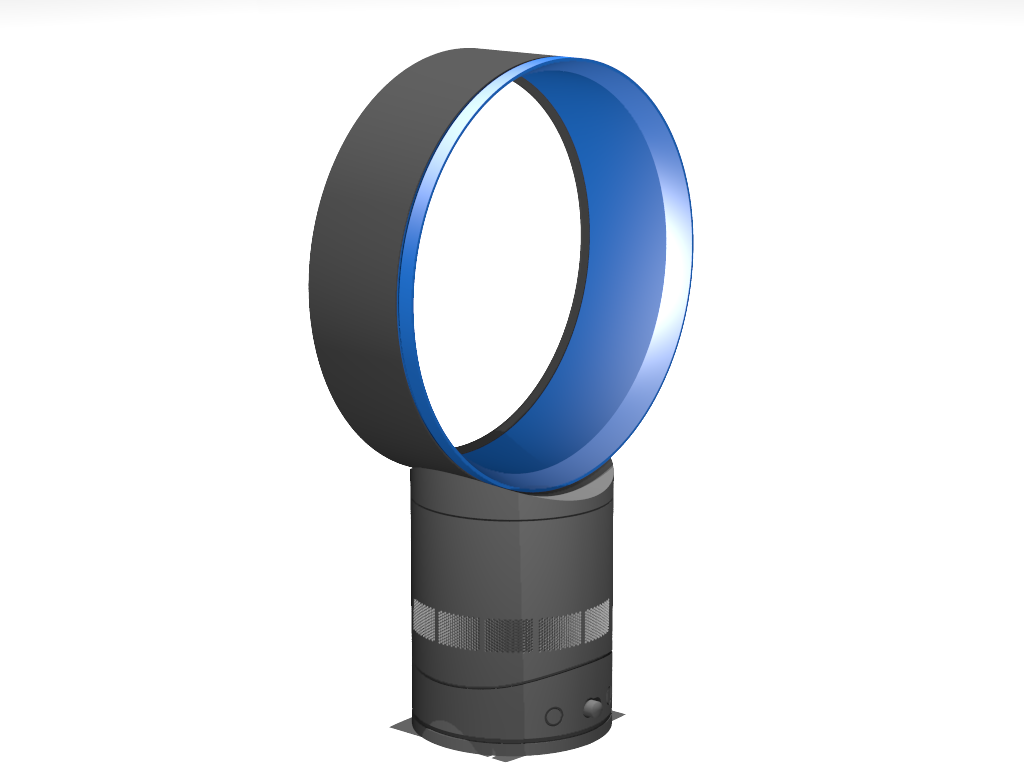
\includegraphics[height=80mm,bb=0 0 1024 768]{POVRAY/dyson.png}
  \figcaption{ダイソン扇風機}
  \label{fig:dyson}
\end{figure}

\section{考察}
\label{sec:考察}

\subsection{完成度}
\label{sub:完成度}
完成度では、まだまだであろうか。
課題としては、素材の感じが出せていないことと、ライティングがもっと工夫できそうであるなと思われる。

\subsection{送風部}
\label{sub:送風部}

送風部は色がオリジナルのものをなかなか再現できなかった…ライティングなどでも大きく色味が変わってしまうため、
最適な色を探すことに苦労した。

\subsection{筒部}
\label{sub:筒部}
筒の部分では、CSG木を大量に用いて、遠山量が増えすぎてしまい、思うように調整するのに多量の時間を取られてしまった。
真ん中の、外気を吸うためのメッシュ状の穴を再現するのがとても大変であった。
全体として、角を取ることができなかったので、まだまだ改善の余地はあると思われる。



\end{document}
